\chapter*{Заключение}                       % Заголовок
\addcontentsline{toc}{chapter}{Заключение}  % Добавляем его в оглавление

%% Согласно ГОСТ Р 7.0.11-2011:
%% 5.3.3 В заключении диссертации излагают итоги выполненного исследования, рекомендации, перспективы дальнейшей разработки темы.
%% 9.2.3 В заключении автореферата диссертации излагают итоги данного исследования, рекомендации и перспективы дальнейшей разработки темы.
%% Поэтому имеет смысл сделать эту часть общей и загрузить из одного файла в автореферат и в диссертацию:

В работе были получены новые важные результаты о квантовых и модифицированных классических бильярдах на софокусных столах.

Исследовано и вычислено симптотическое поведение уровней энергии свободной квантовой частицы в двух областях, ограниченных дугами гипербол и внешнего эллипса, которые при стремлении фокального расстояния к нулю принимают форму кругового сектора при стремлении фокального расстояния к нулю, и вычислен спектр наблюдаемой, соответствующей дополнительному интегралу классической системы.
А именно, в главе 2 получены точные решения стационарного уравнения Шрёдингера в областях $A_\delta$ и $B_\delta$. Вычислена асимптотика собственных значений для близких к нулю фокусных расстояний с точностью до квадрата расстояния. 
Заметим, что предложенный в диссертации метод может быть продолжен на более высокие порядки. Ожидается, что для коэффициентов таким образом могут быть получены аналитические выражения в терминах специальных функций.

Доказана интегрируемость классического бильярда на софокусных столах, разделенных софокусными квадриками на области, заполненные изотропными средами с различными показателями `оптической плотности' при условии, что на границе раздела сред выполняется косинусный закон преломления.
В главе 3 показано, что подчиняющейся косинусному закону преломления классический бильярд на софокусном столе является интегрируемой системой. 
Получена явная формула дополнительного интеграла. Отметим, что в зависимости от параметров квадрик, разделяющих среды, и параметров `оптических плотностей', дополнительный интеграл может оказаться многозначным. 


Исследованы и описаны слоения изоэнергетического многообразия на поверхности постоянного уровня дополнительного интеграла для двух `оптических систем' с косинусным законом преломления, т.е. для софокусных столов, разделенных софокусными квадриками на области, заполненные изотропными средами с различными показателями `оптической плотности'  при условии, что на границе раздела сред выполняется косинусный закон преломления.
А именно, в главах 4 и 5 рассмотрены два примера таких систем, описаны поверхности регулярного значения дополнительного интеграла и перестройки на критических уровнях этого интеграла. 

===============

%
%
%В главе 4 приведено описание поверхностей постоянного уровня интеграла $\Xi$ для бильярда в эллипсе $\Omega = \Omega_1 \cup \Omega_2$ с преломлением согласно косинусному закону на софокусном эллипсе (задача А).
%Приведена методика построения по всей видимости новых бифуркационных  диаграмм, которые учитывают одновременно все возможные значения оптических параметров областей. 
%Получены ранее не встречавшиеся в теории динамических систем особые поверхности, соответствующие одновременным разным бифуркациям в фрагментах бильярдного стола $\Omega_i$. 
%
%Аналогичная задача решена в главе 5 на другом софокусном столе $\Omega = \Omega_1 \cup \Omega_2$ (задача Б). 
%Сложность задачи обусловлена тем, что бильярдная траектория может неоднократно посещать каждый фрагмент $\Omega_i$ с разными параметрами касательной квадрики. 
%В работе это обстоятельство преодолено: найден однозначный интеграл $\Xi$, для которого построена бифуркационная диаграмма, с помощью которой описаны поверхности уровня этого интеграла $\Xi$ для регулярных и критических значений.

В качестве направлений дальнейших исследований можно выделить следующие.
  \begin{itemize}[beginpenalty=10000] % https://tex.stackexchange.com/a/476052/104425
  \item Построение аналогичных асимптотик уровней энергии квантового бильярда в присутствии потенциала.
  \item Изучение квантовых бильярдов для более широкого класса областей. Применение изложенных в диссертации методов позволяет вычислить асимптотику собственных значений для квантового бильярда в <<эллиптическом прямоугольнике>> (см. рис. \ref{fig:conclusion_quantum_domains}). Существуют иные <<эллиптические секторы>>, которые при сближении фокусов также стремятся к круговому сектору, но для анализа задач в них требуется продвинутое понимание распределения нулей  угловых функций Матьё.
    \begin{figure}[ht]
    \centerfloat{
        \hfill
        \subcaptionbox{<<эллиптический сектор>>}{%
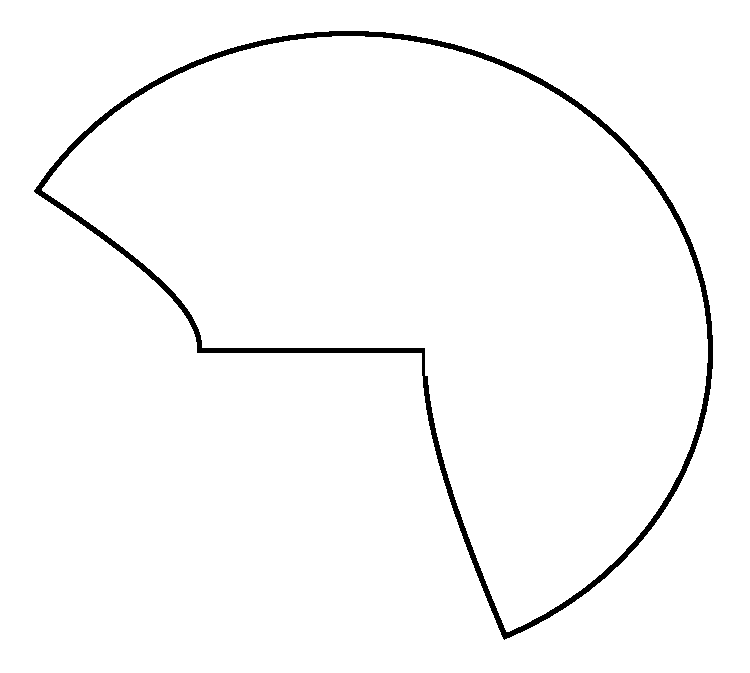
\includegraphics[width=3.5cm]{future/future_1.pdf}}
        \hfill
        \subcaptionbox{<<эллиптический прямоугольник>>}{%
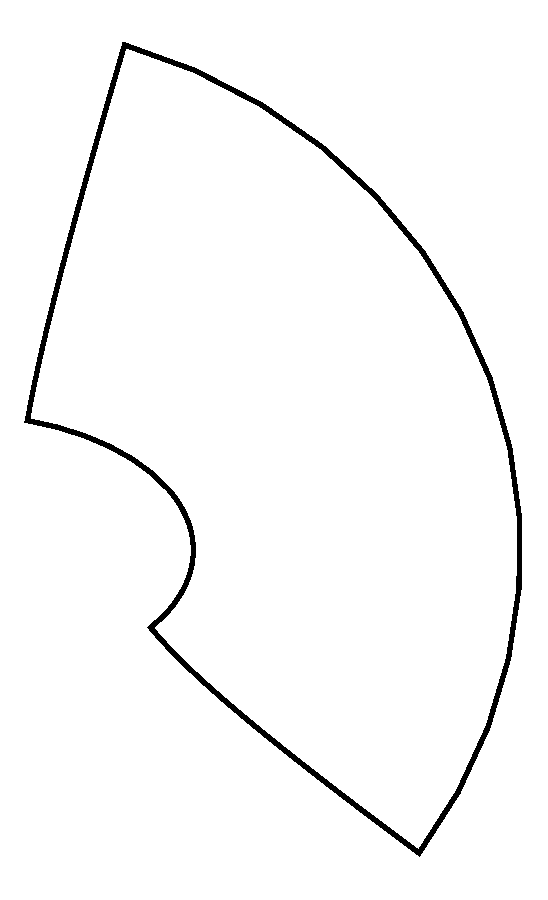
\includegraphics[width=2.5cm]{future/future_2.pdf}}
        \hfill
    }
    \caption{Софокусные столы для перспективных квантовых задач.}\label{fig:conclusion_quantum_domains}
\end{figure}  
  \item Исследование `оптического бильярда' для других разбиений бильярдного стола.
  \item Изучение бильярдных книжек с косинусным законом преломления. При этом границы раздела сред могут проходить не только внутри листов, но и вдоль корешков. 
  \item Вычисление инвариантов Фоменко-Цишанга для оптических бильярдов с косинусным законом преломления.
  \end{itemize}

%%% Согласно ГОСТ Р 7.0.11-2011:
%% 5.3.3 В заключении диссертации излагают итоги выполненного исследования, рекомендации, перспективы дальнейшей разработки темы.
%% 9.2.3 В заключении автореферата диссертации излагают итоги данного исследования, рекомендации и перспективы дальнейшей разработки темы.
\begin{enumerate}
  \item Логичным продолжением представленного исследования \ldots
\end{enumerate}

